\newpage
\subsection{Учет технологической оснастки и краски }
\label{bp:rigging}
%
Технологическая оснастка необходима для изготовления готовой продукции. На предприятии заказывают оснастку у сторонних производителей.

При получении требований от клиента менеджер определяет необходимость использования оснастки при производстве продукции. 

Возможность изготовления нового изделия, в соответствии с техническими параметрами оборудования, определяет главный технолог. 




\textbf{Учет клише}

Дизайнер, на основании разработанного и согласованного дизайна заказывает изготовление клише. 

Предприятие использует одного поставщика клише. 
Для размещения заказа на изготовление клише дизайнер отправляет макет по электронной почте.

Учет количества размещенных заявок на изготовление клише не ведется. 
При изготовлении клише за счет клиента менеджер создает запрос в бухгалтерию для выставления счета. Бухгалтер выставляет счет на изготовление оснастки.

При поступлении на производство клише проверяется на соответствие макету, фиксируется дата поступления в MS EXCEL (рис. \ref{pic:f17}). Кладовщики о факте поступлении оснастки сообщают дизайнерам. 

Номер клише присваивает дизайнеры в момент заказа у поставщика.

На предприятии выделен участок для хранения клише.


\textbf{Учет штанцевальных форм}

 Менеджер передает в отдел дизайна макет штампа. Далее данный макет обрабатывается и отсылается главному технологу. Главный технолог чертит раскладку на штампе и прописывает оборудование, возвращает дизайнерам. Далее дизайнеры отсылают раскладку с макетом поставщику штампов и заказываю штамп.

Компания-изготовитель оснастки выставляет счет. Если изготовление штанцевальной формы выполняется за счет клиента, то менеджер делает запрос в бухгалтерию на выставление счета. Бухгалтер выставляет счет покупателю.

При поступлении штампа на производство  штамп проверяется. 

Номер присваивают дизайнера в момент заказа .

На предприятии места для хранения штампов оборудованы рядом с перерабатывающими линиями. Предусмотрена ячеистая система хранения. 

Учет штанцевальных форм ведется MS EXCEL, где указывается номер штампа и номер ячейки хранения (рис. \ref{pic:f22}).

Ремонтом оснастки занимаются в основном на производстве. Учет объема выполненных ремонтных работ не ведется.


Журнала выдачи оснастки не обнаружено.




%\subsubsection{Учет печатных форм}




%\subsubsection{Изготовление штампов}




\textbf{Учет краски}

Колорист получает задание на смену для каждой отдельной линии (рис. \ref{pic:f18}), подбирает технологические карты, по которым определяет номера краски, планируемой в работу. Колорист <<по своему опыту>> готовит краску на заказ (рецептура используется номинально). 

После приготовления краску выдают на линию. Учет краски колорист ведет в MS EXCEL (рис. \ref{pic:f19} - рис. \ref{pic:f20}). Общий итог расхода определяется по таблице MS EXCEL (рис. \ref{pic:f21}).

\begin{figure}
\begin{center}
 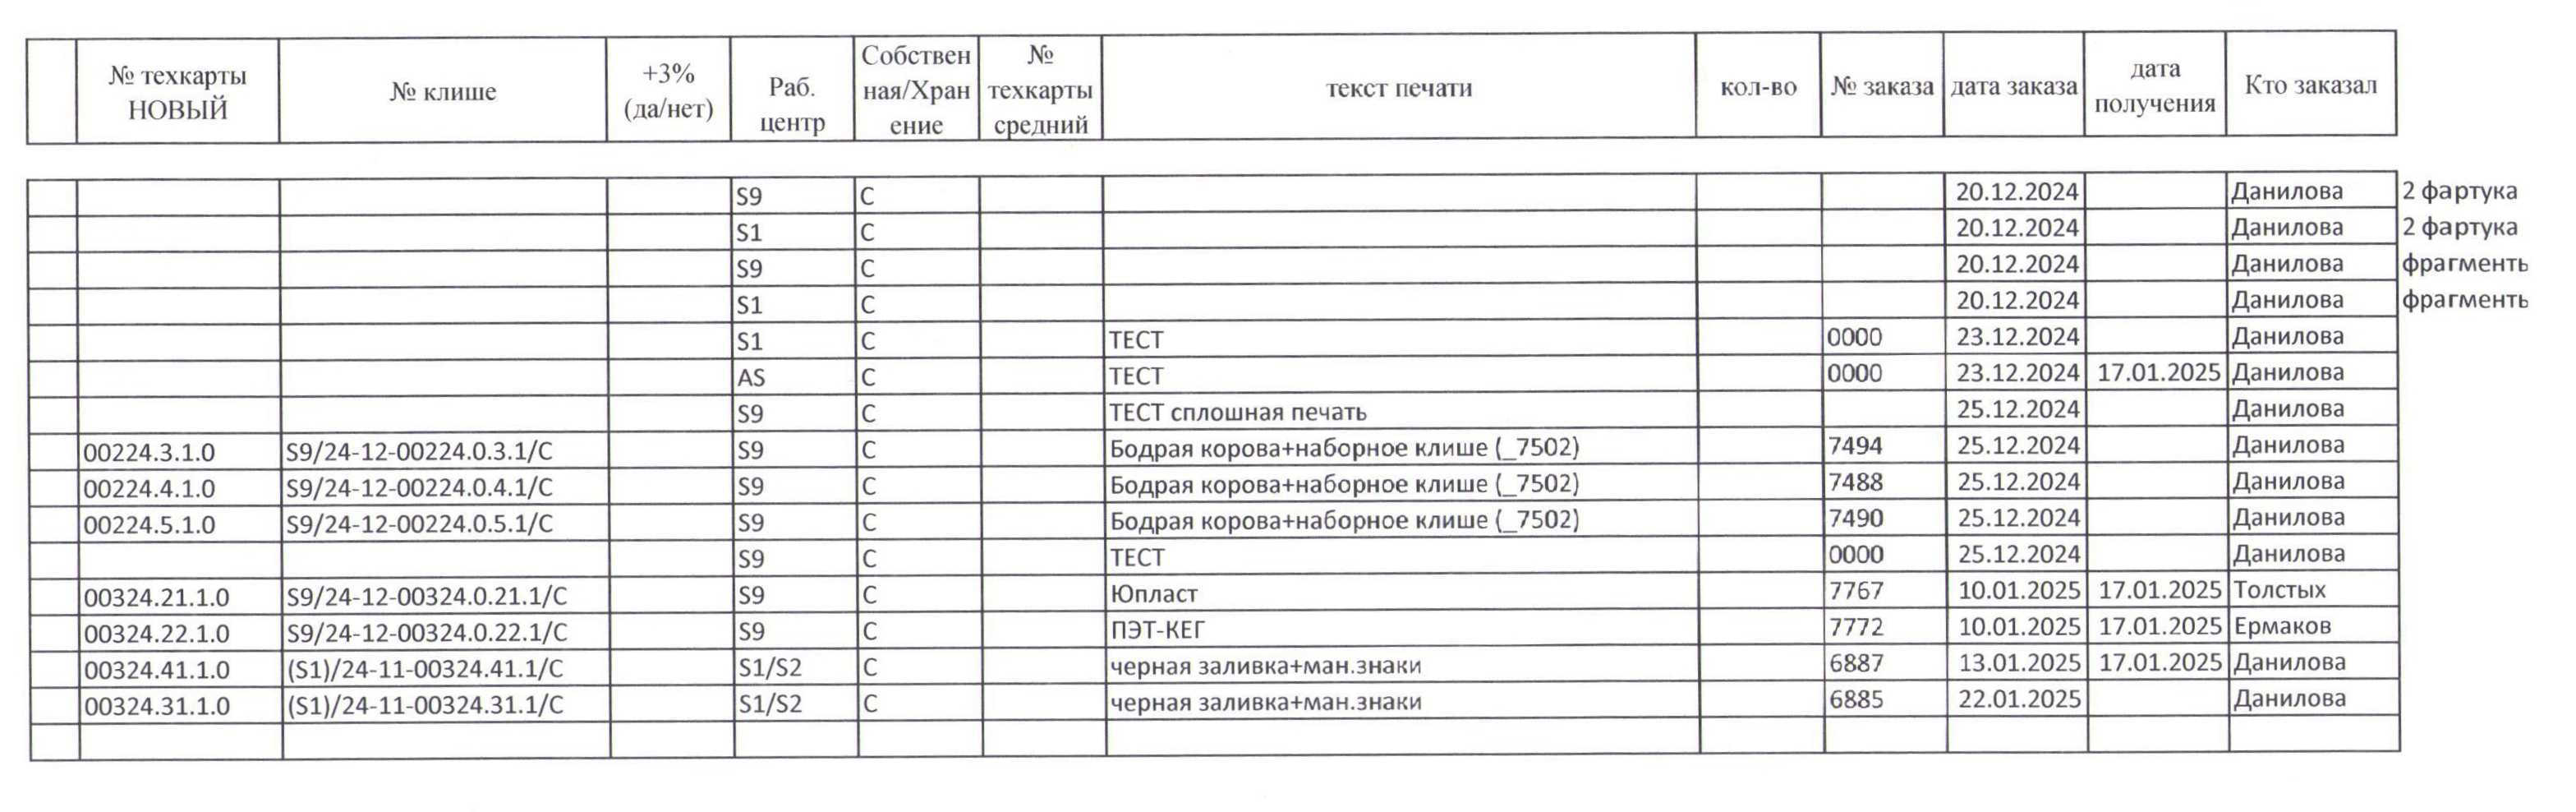
\includegraphics[width=\linewidth, height=0.94\textheight, angle=90, keepaspectratio]{Pics/f17.jpg}
\end{center}
\caption{Электронный реестр клише}
\label{pic:f17}
\end{figure}

\begin{figure}
\begin{center}
 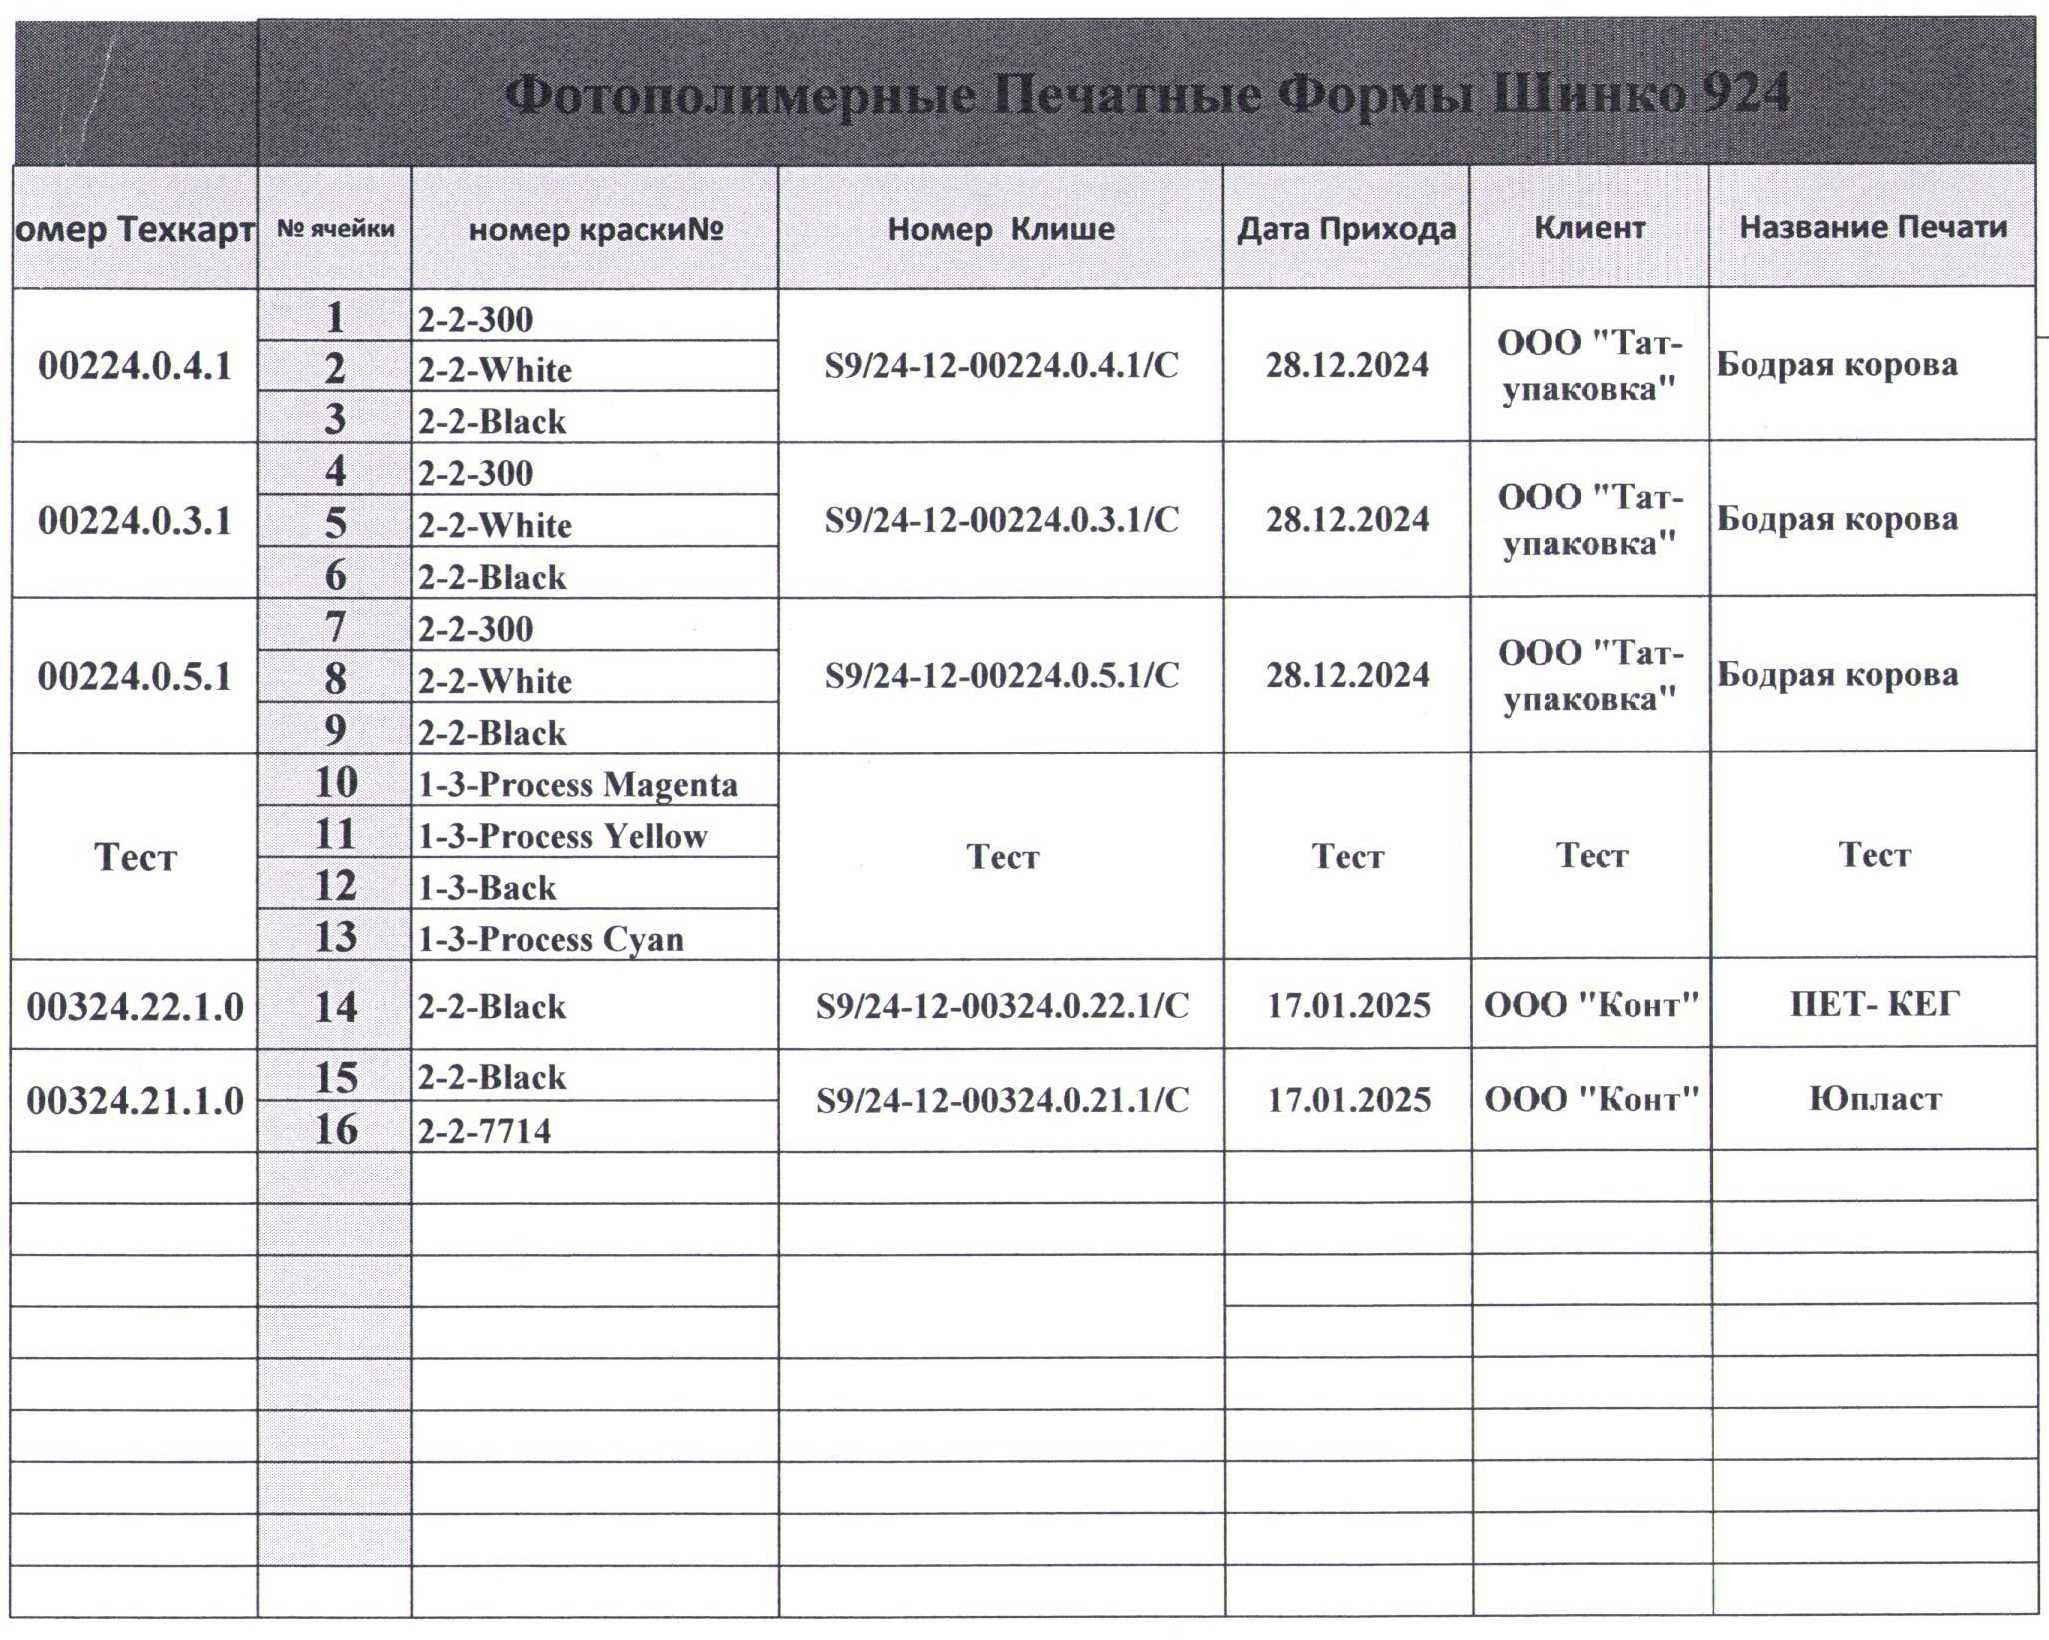
\includegraphics[width=\linewidth, height=0.94\textheight, keepaspectratio]{Pics/f22.jpg}
\end{center}
\caption{Каталог размещения клише в ячейках}
\label{pic:f22}
\end{figure}

\begin{figure}
\begin{center}
 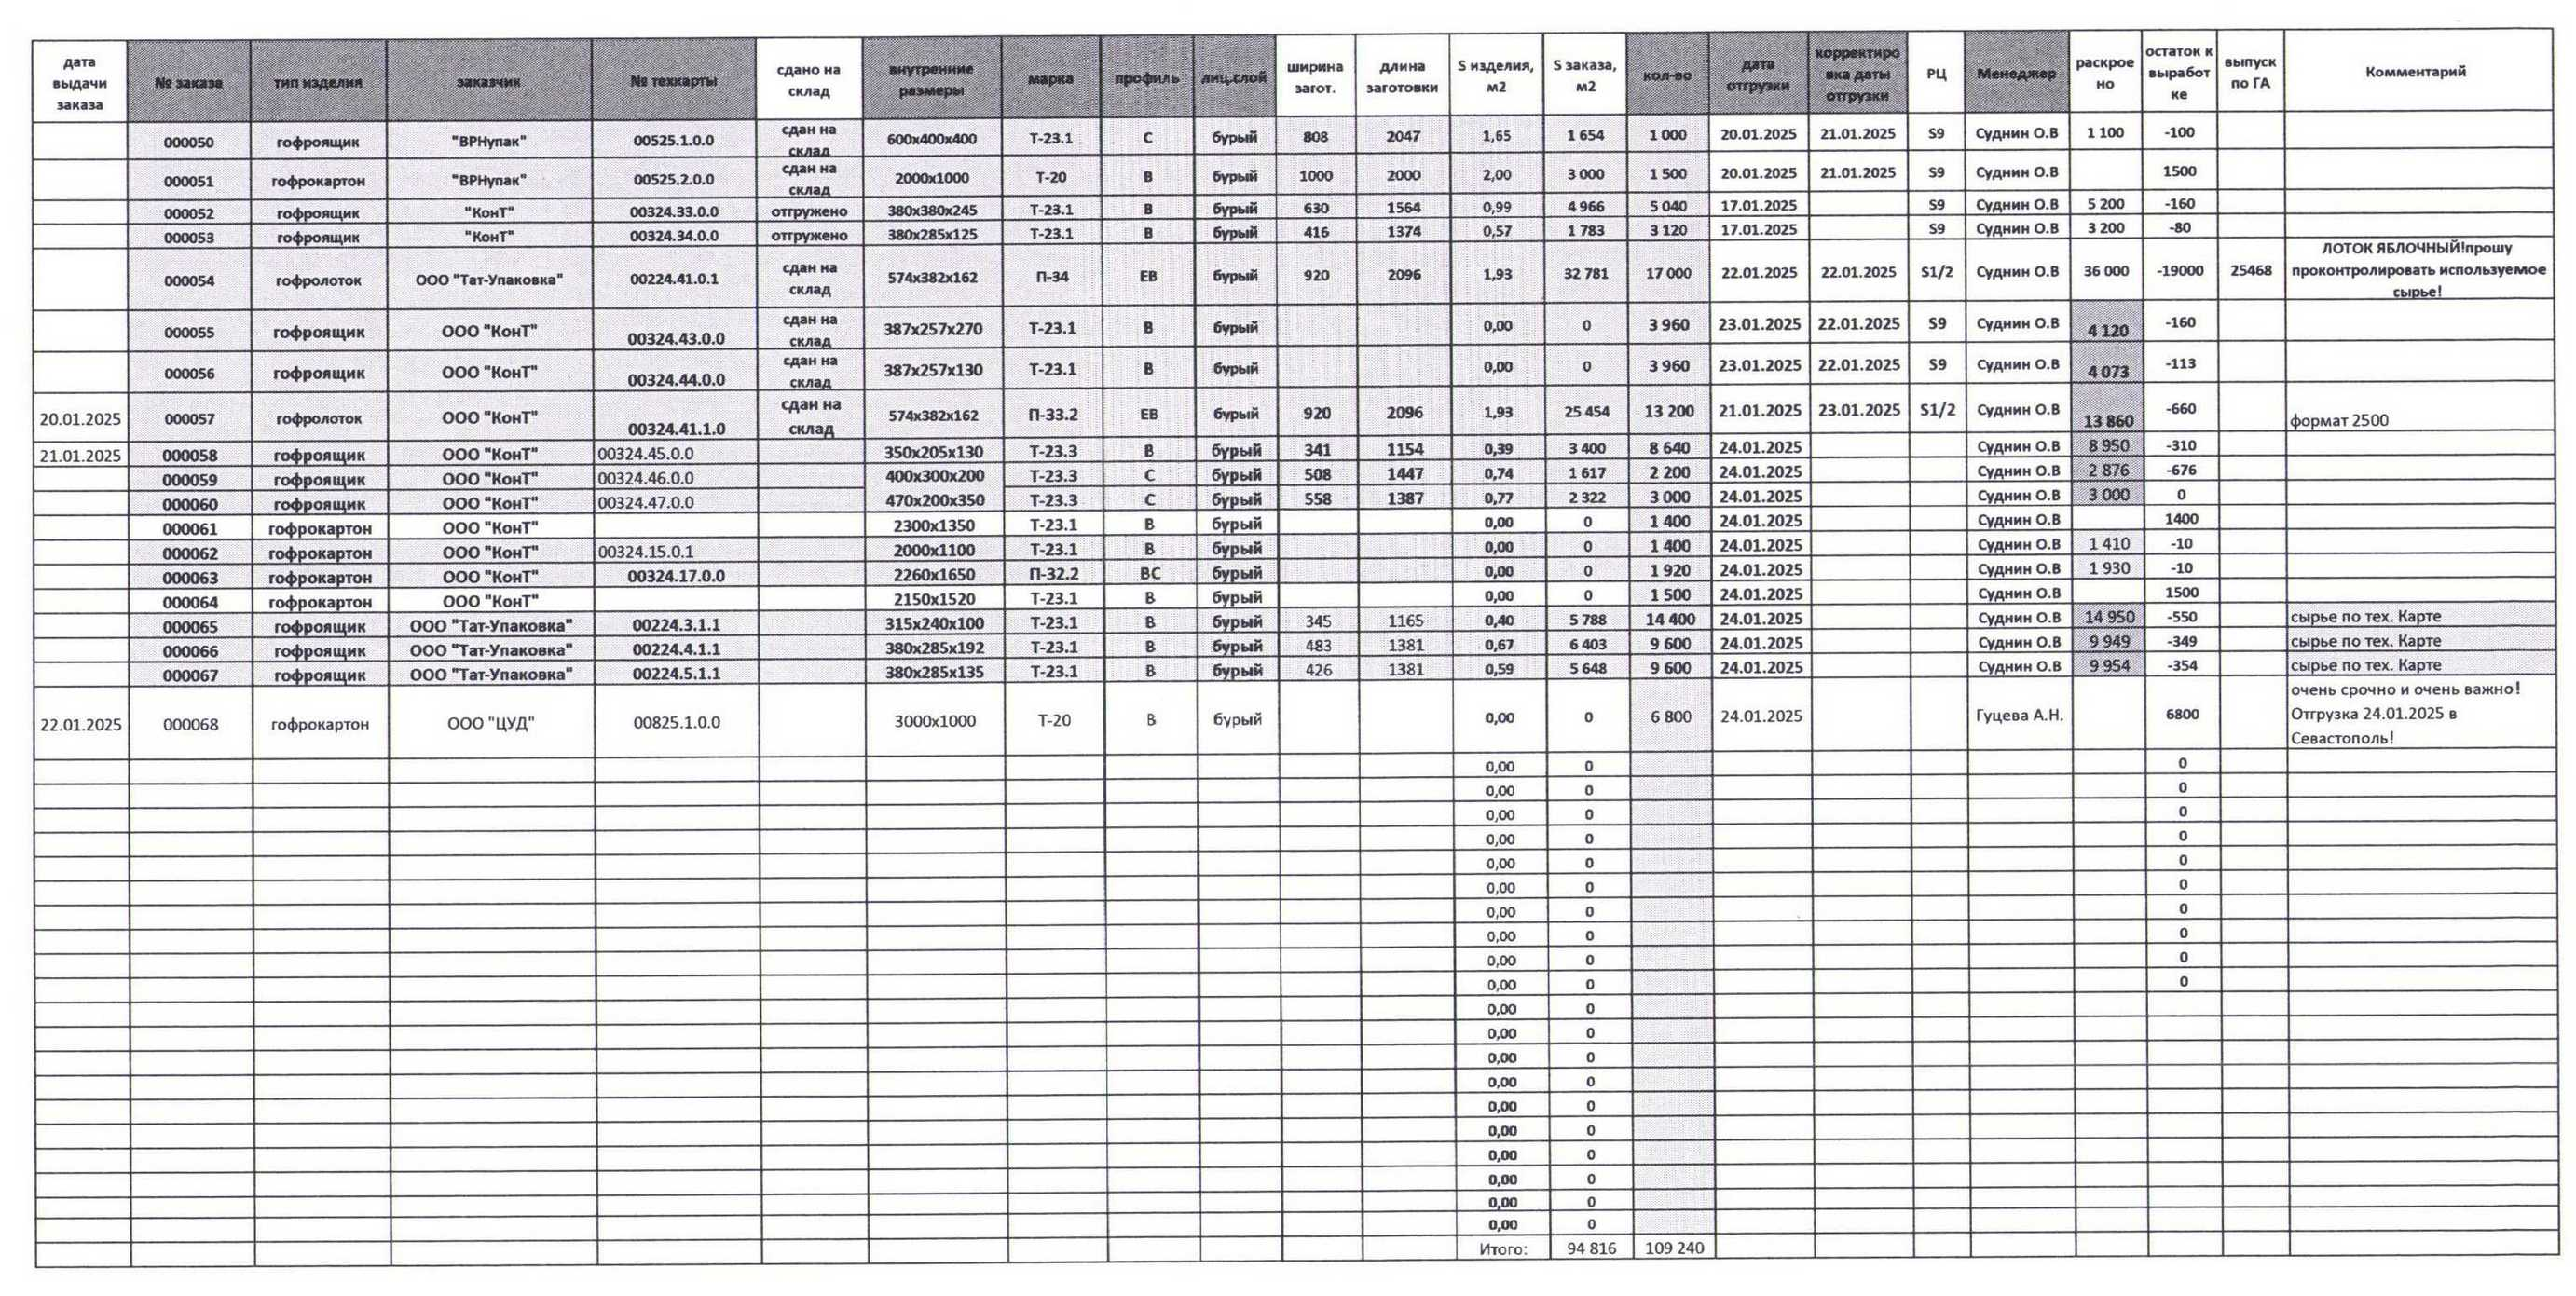
\includegraphics[width=\linewidth, height=0.94\textheight, angle=90, keepaspectratio]{Pics/f18.jpg}
\end{center}
\caption{Задание на смену для колориста}
\label{pic:f18}
\end{figure}

\begin{figure}
\begin{center}
 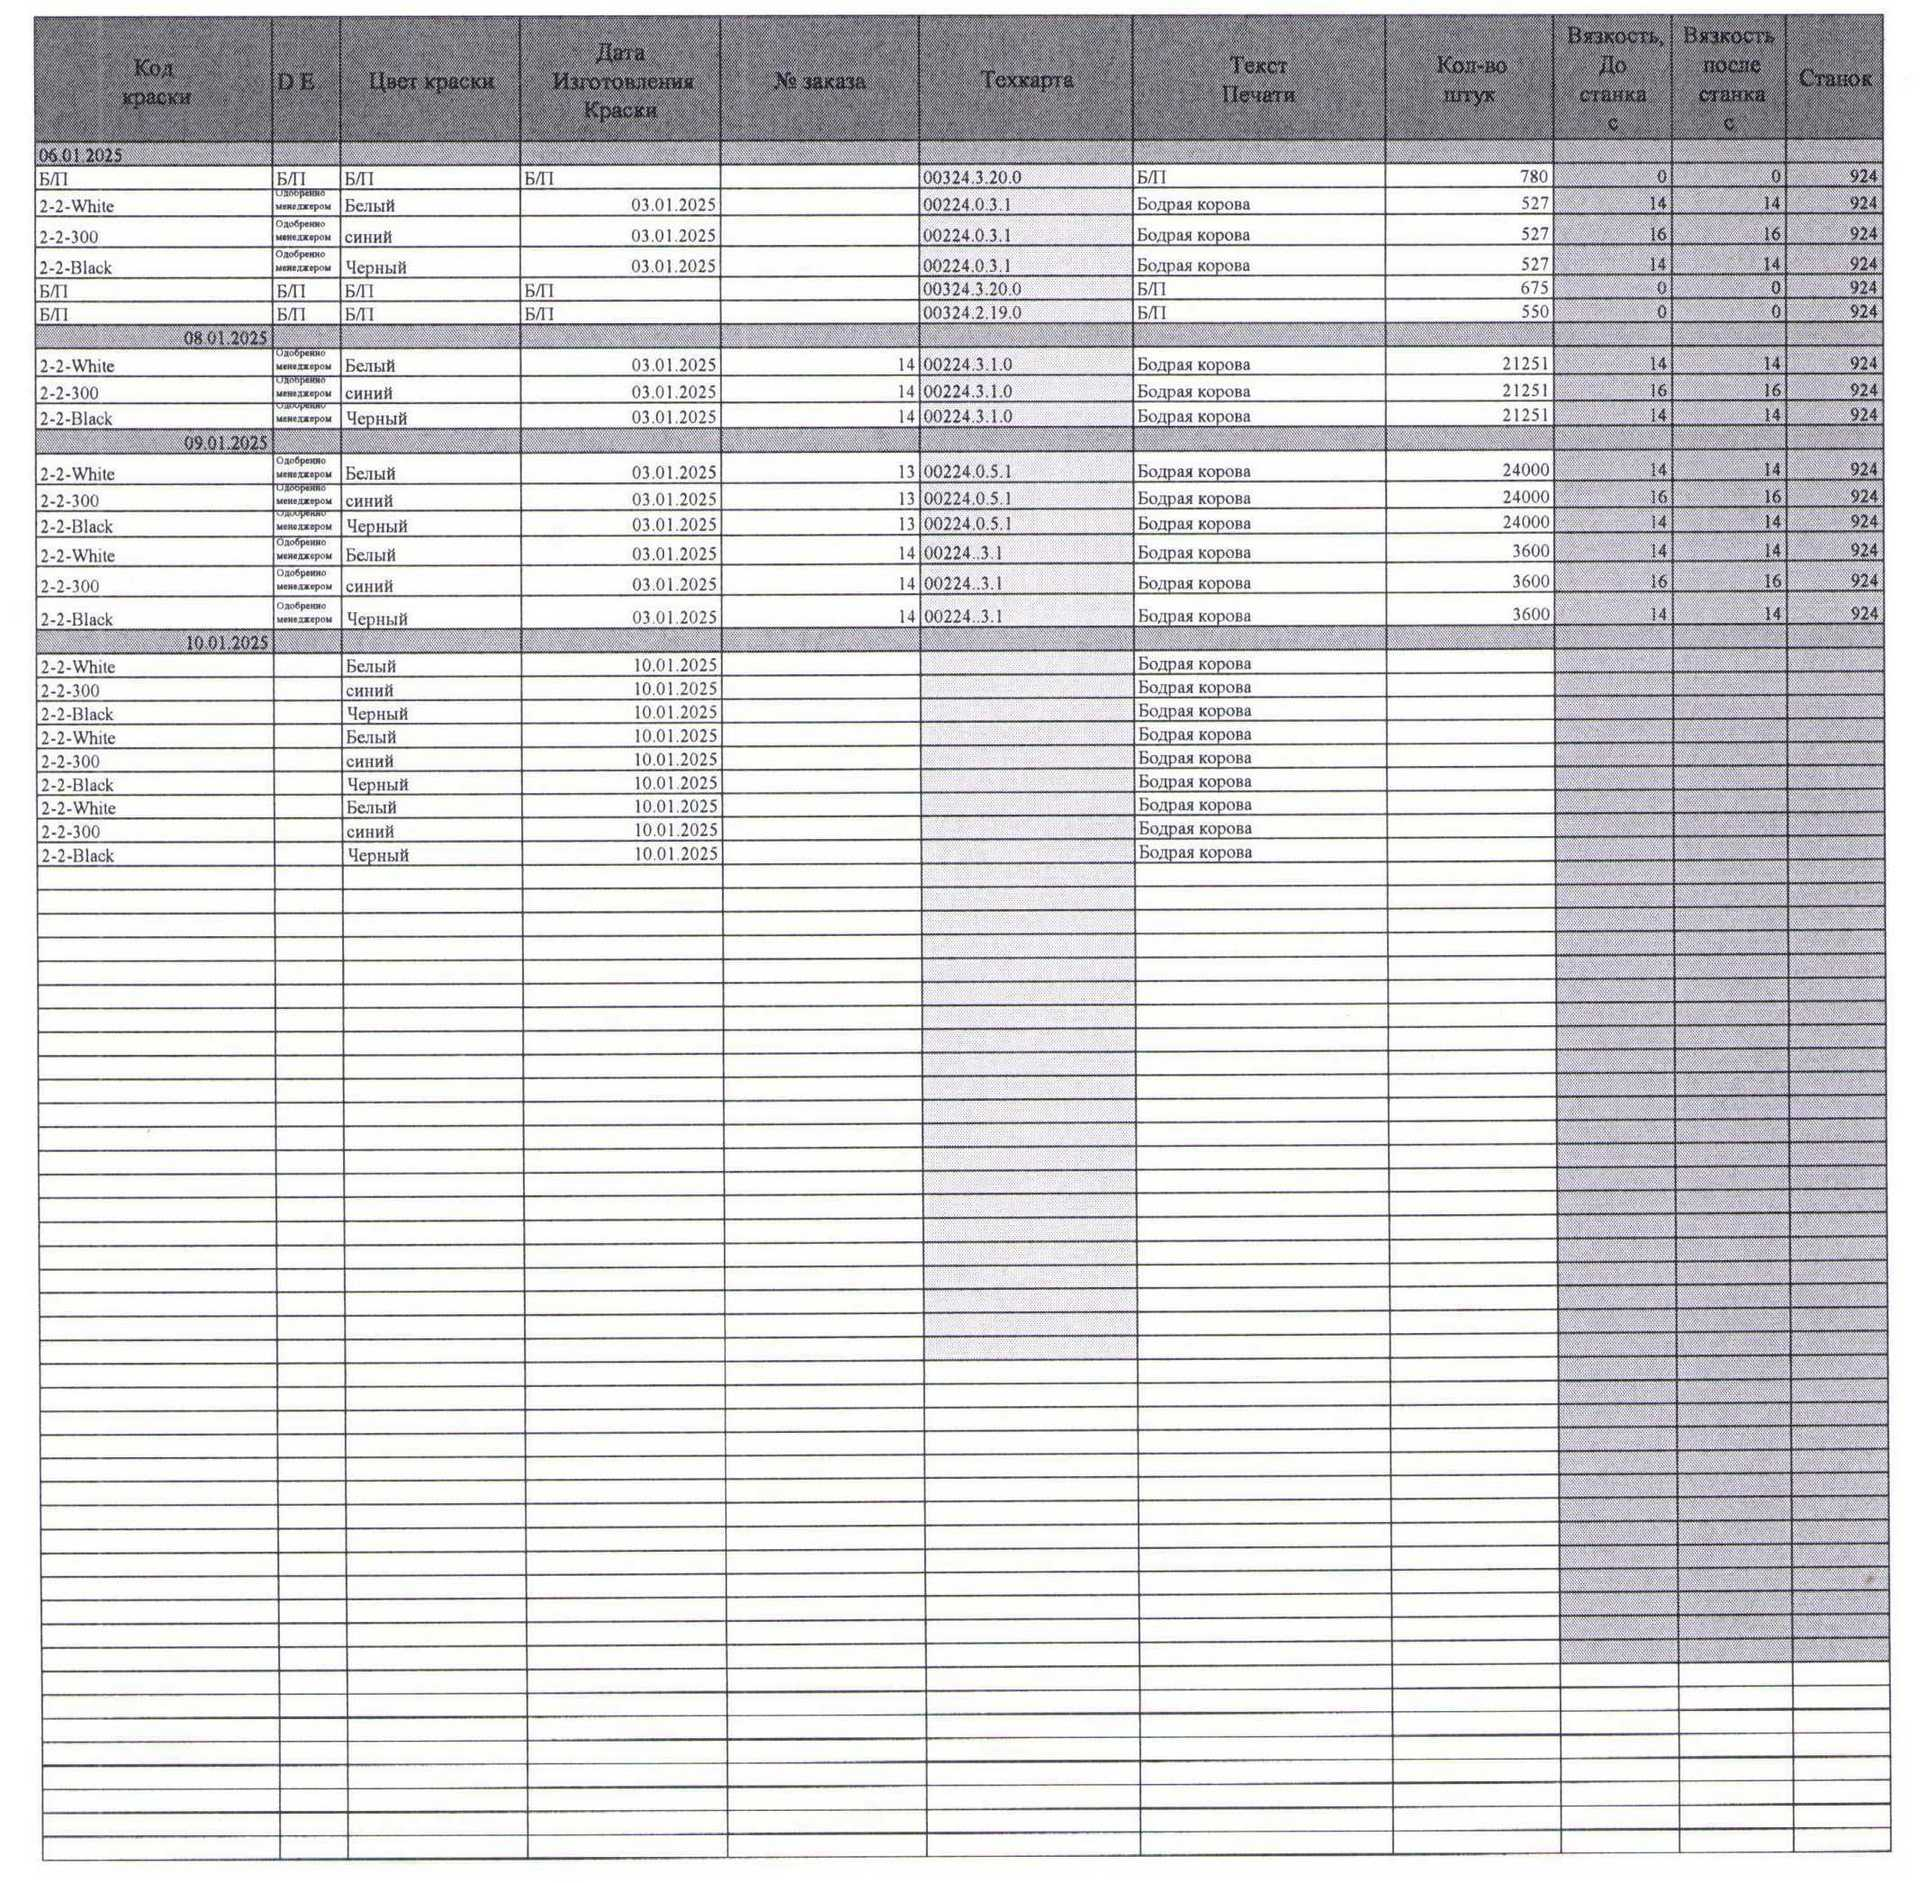
\includegraphics[width=\linewidth, height=0.94\textheight, angle=90, keepaspectratio]{Pics/f19.jpg}
\end{center}
\caption{Учет выдачи готовой краски на производство. Часть 1}
\label{pic:f19}
\end{figure}

\begin{figure}
\begin{center}
 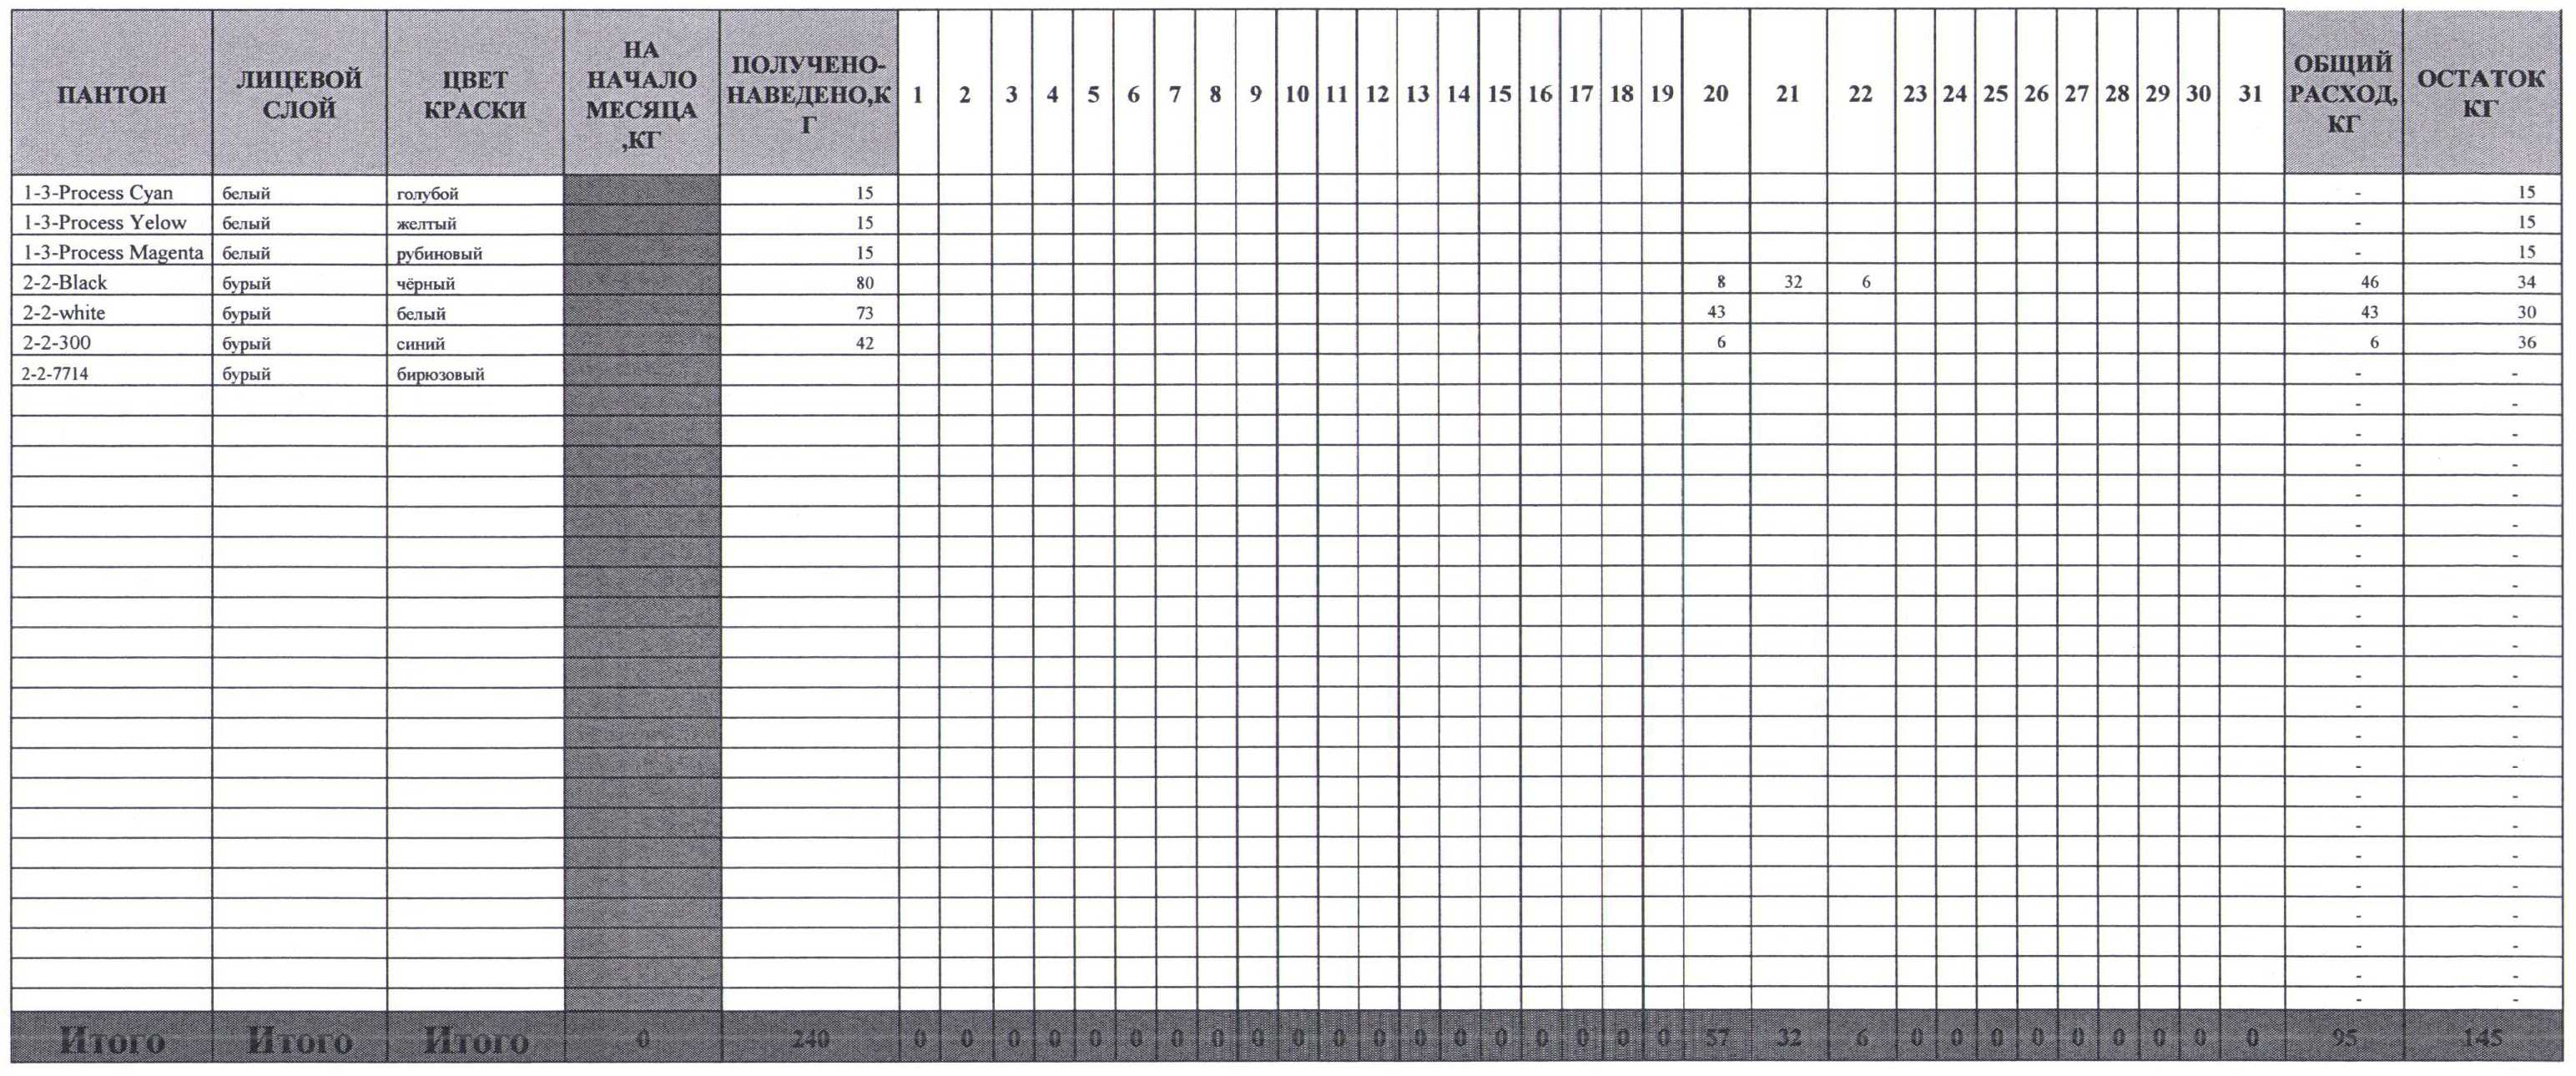
\includegraphics[width=\linewidth, height=0.94\textheight, angle=90, keepaspectratio]{Pics/f20.jpg}
\end{center}
\caption{Учет выдачи готовой краски на производство. Часть 2}
\label{pic:f20}
\end{figure}

\begin{figure}
\begin{center}
 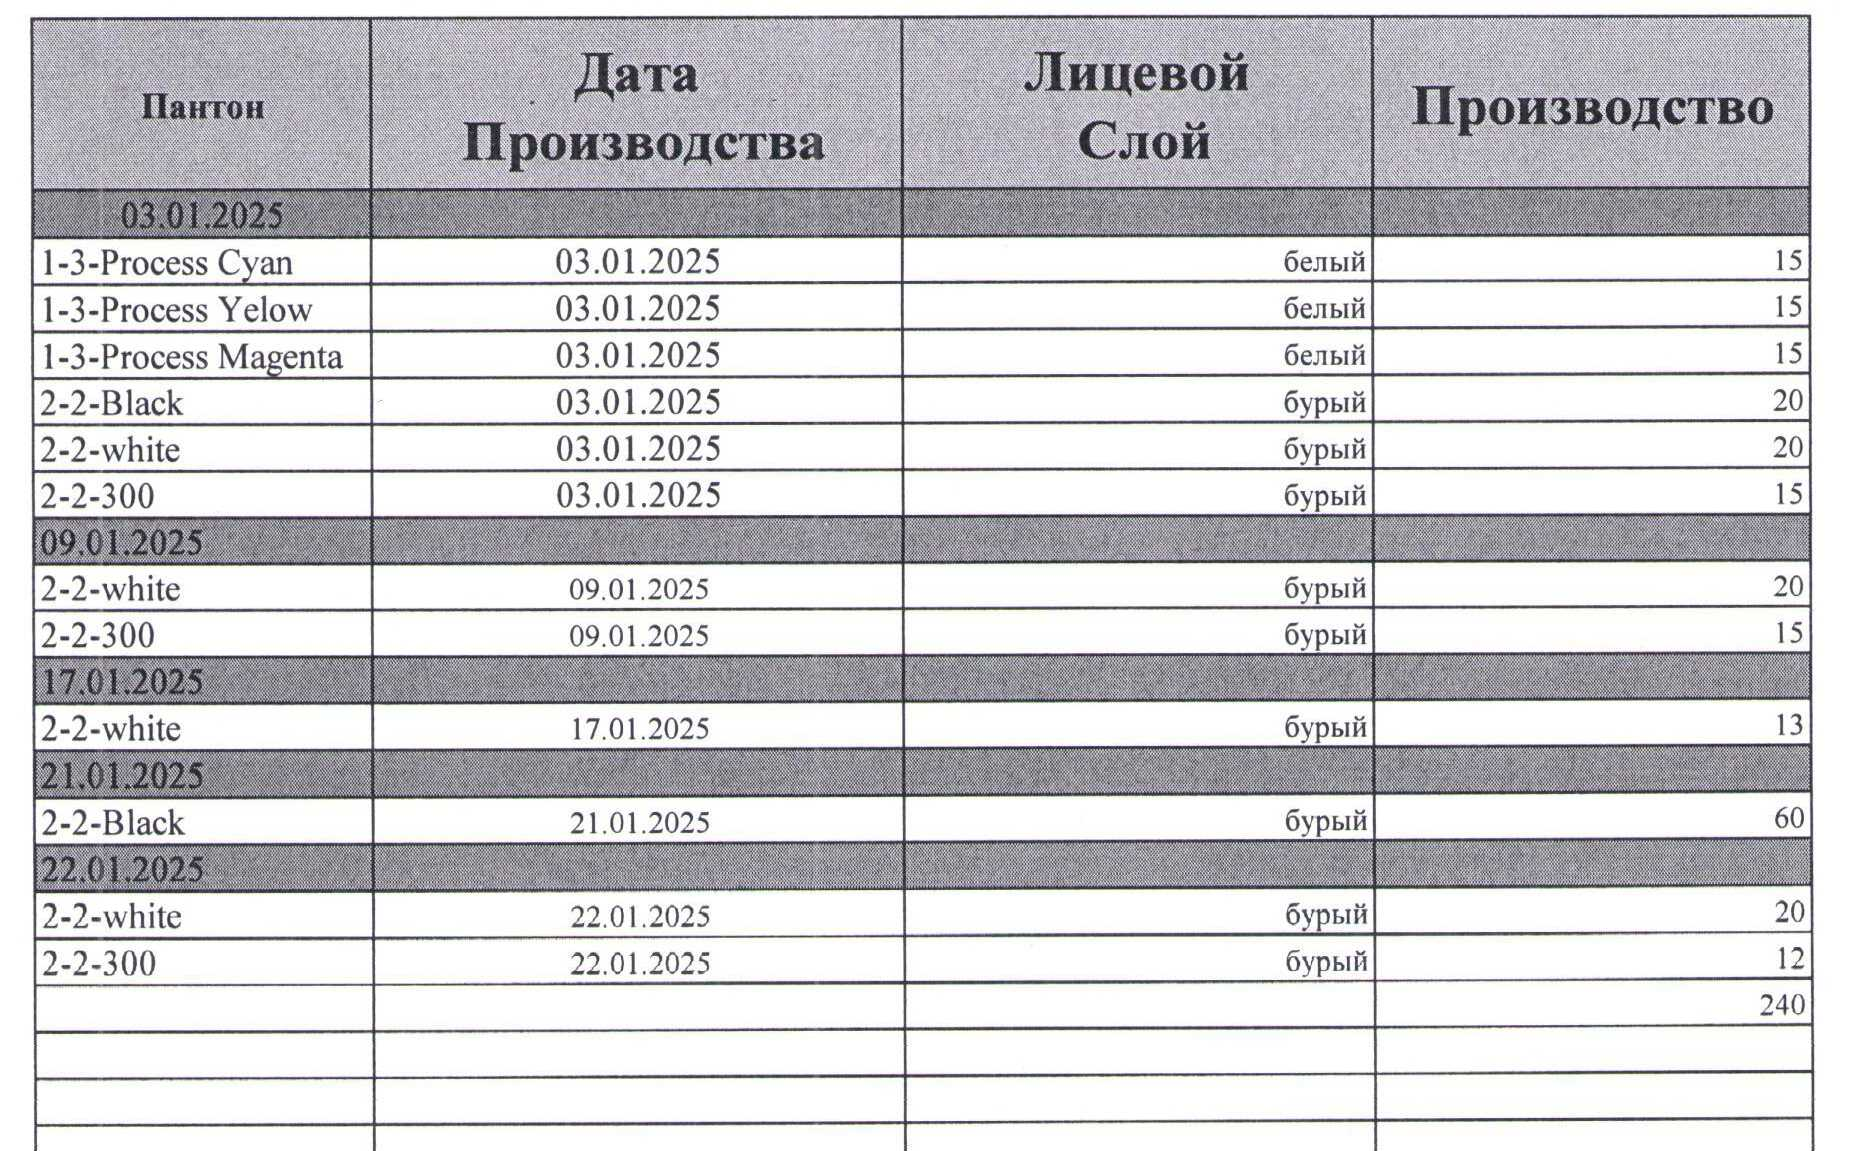
\includegraphics[width=\linewidth, height=0.94\textheight, keepaspectratio]{Pics/f21.jpg}
\end{center}
\caption{Баланс по краске}
\label{pic:f21}
\end{figure}




\clearpage
\ifx \notincludehead\undefined
\normalsize
\end{document}
\fi
